\chapter{OpenCL}
\label{ch:OpenCL}
This chapter serves as an overview of OpenCL, an open and royalty-free standard for parallel programming on heterogenous systems.
Topics that are important for the understanding of implementations presented in this thesis will be emphasized.
In addition, a more thorough study of matrix multiplication is presented, as well as historical aspects on GPGPU computing.


\section{General-purpose computing on GPU}
With the continuous emergence of new graphic cards, high computational powers reaches consumers, ranging from regular desktop users to HPC users.
Whereas regular processors have powers in the range of 10 to 100 gigaflops, graphic cards can reach more than teraflops performance.
As an example the AMD radeonhd 6970, which is used extensively in this thesis, is listed with a speed of 2.7 TFLOPs for single precision, and 683 GFLOPs for double precision \cite{radeon6970}.
Having a price of a few thousand NOK, graphical processing units (GPUs) can compare with larger clusters having a much higher price.

\paragraph*{}
GPUs were originally, and still are, targeted mainly towards computer graphics.
To be able to produce real time graphics with a high level of detail, such a processor must be highly parallel.
A large amount of pixels is needed within a short time range.
However, since higher framerates than 30-60 frames per second are often unnecessary for the human eye, the need for high frequencies are set aside for greater number of processing units.

Some programmers did eventually see the potential of GPUs to paralellize and accelerate general purpose programs, but the lack of standards for this forced them to translate problems into a graphics-like problem in order to run them on GPUs.
Video cards also lacked hardware features making it even harder to program general code on them.
Even today double precision arithmetics are supported mostly on high-end cards, and require the latest drivers.

\paragraph*{}
To overcome the issues of GPU computing, a few standards arose.
At the moment three major standards exists; DirectCompute, CUDA and OpenCL.
All of them supply a language for writing accelerated code, as well as an API to control the execution of this code.
The first two standards will not be used in this thesis, mainly because of their lack of choice.
Whereas DirectCompute enforces the use of Microsoft Windows and CUDA limits itself to NVIDIA cards, OpenCL have implementations on all common\footnote{Implementations exists at least for recent versions of Windows, Mac and Linux} operating systems for both CPUs and GPUs from Intel, AMD and NVIDIA.



\section{The OpenCL model}
The OpenCL standard~\cite{openclspec} describes OpenCL with the following hierarchy of models:
\begin{itemize}
\item Platform model
\item Memory model
\item Execution model
\item Programming model
\end{itemize}


\subsection{Platform model}
OpenCL programs consists of a host running code written in C/C++.\footnote{The OpenCL API is written in C with bindings for C++. Third party wrappers can still be found for other languages. See for example JOCL or javaCL for java, and pyopencl for python implementations.}
This host have access to different devices, each consisting of a number of compute units with one or more processing elements.

The simplest setup would consist of a single threaded host program running on the CPU. 
By querying for a platform and a device it can gain access to the CPU. 
This may seem illogical, but it is an easy way to program parallel on the processor.
A quad core, which is common, would typically permit four compute units (four \textit{independent} threads), with one processing element each.

A slightly more advanced configuration could consist of the simple setup, but also have access to the video card.
The GPU would now show up as a second device, having e.g. 24 compute units (SIMD cores) with 64 processing elements each. Whereas the compute units run independently, the processing elements within a compute unit will generally not.
This hierarchy is defined by the platform model.

\begin{figure}
\begin{center}
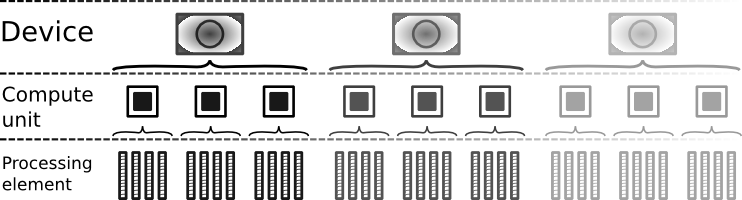
\includegraphics[scale=0.5]{../08-OpenCL/figs/platform.png}
\caption{The hierarchy defined by the OpenCL platform model.
A platform consists of multiple devices, each having multiple compute units. Whereas compute units can run independent threads, they can still contain multiple processing elements.
The memory model (\ref{sec:OpenCL:memmodel}) will also fit in this hierarchy, with (from the top) global, local and private memory residing close to corresponding layer.}
\label{fig:OpenCL:platform}
\end{center}
\end{figure}


\subsection{Execution model}
Code is written in its own language `.cl' which is a subset of the C99 standard, where functions callable from the host are called kernels.
This code is then compiled for an already initialized device, and submitted to a command queue.
The command queue is now responsible for running this kernel once the device is ready. 
It is possible to submit multiple kernels to a queue and manage their execution via events.

\paragraph*{}
Every time a kernel is queued, a virtual grid will be defined.
For every grid point, the kernel will be executed once.
This is how parallelism is achieved in OpenCL.
This so-called NDRange can be of one, two or three dimensions, and the size can be chosen arbitrarily up to a limit defined per device.

The entire global grid is divided into smaller local grids called work-groups.
An illustration of a 27x27 `2DRange' composed of nine 9x9 workgroups is found in figure~\ref{fig:OpenCL:ndrange}.
During execution each work-item will fill one processing element.
All work-items within the same work-group will run concurrently, but on the same compute unit. The other work-groups will run on other compute units within the same device.

\begin{figure}
\begin{center}
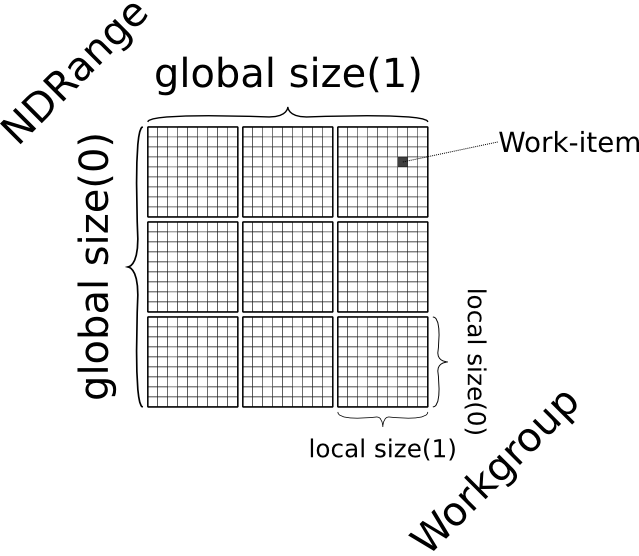
\includegraphics[scale=0.5]{../08-OpenCL/figs/NDRange.png}
\caption{A global two dimensional 27x27 NDRange. It is divided into nine work-groups, each having 9x9 work-items.}
\label{fig:OpenCL:ndrange}
\end{center}
\end{figure}



\subsection{Memory model}
\label{sec:OpenCL:memmodel}
There are four different regions for OpenCL memory:
\begin{itemize}
\item \textbf{Global} memory is allocated by the host. Both kernel and the host have read/write access. The slowest type of memory, but having a large memory size. Ideal for storing matrices or per work-item results.
\item \textbf{Constant} memory is allocated by the host, but kernels have read access only. Often used when passing many parameters/options as one struct to the kernel.
\item \textbf{Local} memory could be allocated either dynamically by the host or statically inside a kernel. Every work group share its own independent copy of this memory type. This memory is faster than global, because it resides close to each compute unit. 
\item \textbf{Private} memory is allocated statically by each work-item and not shared at all. Being closest to each processing item it is the fastest memory. Variables declared in kernels without specifying the region is private by default.
\end{itemize}
A quick summary of the different memory regions can be found in table~\ref{tab:OpenCL:memory}.

\begin{table}
\begin{center}
\begin{tabular}{c|cc|cc|cc|cc}
& \multicolumn{2}{c|}{Global} & \multicolumn{2}{c|}{Constant} & \multicolumn{2}{c|}{Local} & \multicolumn{2}{c}{Private}\\
& Host & Kernel& Host & Kernel& Host & Kernel& Host & Kernel \\
\hline
Allocation & Dyn & NA & Dyn & NA & Dyn & Stat & NA & Stat\\ 
Access & R/W & R/W & R/W & R & NA & R/W & NA & R/W\\ 
\hline 
\end{tabular} 
\caption{Overview of different OpenCL memory regions. R/W: read and write. R: read only. Dyn/Stat: dynamic/static. NA: not available.}
\label{tab:OpenCL:memory}
\end{center}
\end{table}



\subsection{Programming model}
OpenCL focuses on a data parallel programming model.
Here we have multiple memory objects that can be calculated or altered by the same set of instructions. 
Instead of using loops or nested loops, our problem can be simplified by choosing appropriate global and local sizes, as we shall see for general matrix multiplication in section~\ref{sec:OpenCL:matmult}.

Task parallel programming, and hybrids between these two, are also supported. 
GPUs however favors the data parallel model.




\section{GPU architecture}
\label{sec:OpenCL:GPUarchitecture}




\section{Matrix multiplication}
\label{sec:OpenCL:matmult}
The coupled cluster code has its bottleneck in matrix matrix multiplication.
Take for instance the second term of \eqref{eq:CC:t2eq},
\begin{equation}
t_{ij}^{ab} \leftarrow \frac{1}{2} \langle ab||de \rangle t^{de}_{ij} .
\end{equation}
Gathering indices $a,b \rightarrow \alpha$, $d,e \rightarrow \beta$ and finally $i,j \rightarrow \gamma$, it can be rewritten as
\begin{equation}
t_{\alpha,\gamma} \leftarrow \frac{1}{2} \sum_{\beta} \langle \alpha||\beta \rangle t_{\beta,\gamma} ,
\end{equation}
which is, apart from the factor $\frac{1}{2}$, identical to the mathematical definition of matrix multiplication,
\begin{equation}
C_{ij} = \sum_k A_{ik} B_{kj},
\hspace{10mm}
A \in \mathbf{R}^{m\times p}, B \in \mathbf{R}^{p\times n}, C \in \mathbf{R}^{m\times n}.
\end{equation}
Element $C_{ij}$ is thus the innerproduct of row $i$ in $A$ and column $j$ in $B$, as illustrated in fig.~\ref{fig:OpenCL:matmult}.


\begin{figure}
\begin{center}
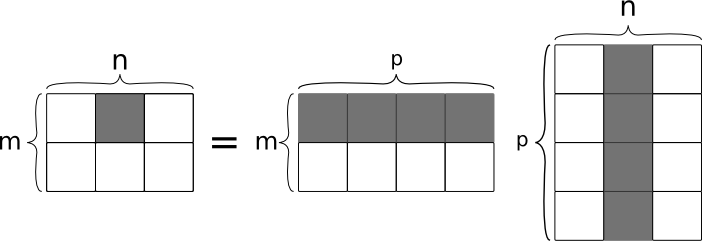
\includegraphics[scale=0.5]{../08-OpenCL/figs/matmult.png}
\caption{Outline of matrix multiplication, following its straight forward mathematical definition.}
\label{fig:OpenCL:matmult}
\end{center}
\end{figure}


\begin{figure}
\begin{center}
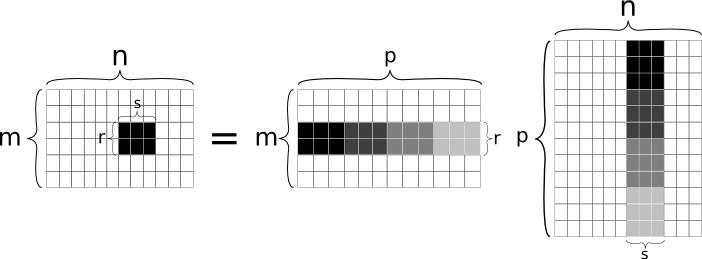
\includegraphics[scale=0.5]{../08-OpenCL/figs/matmult_loc.png}
\caption{Outline of blocked matrix multiplication.}
\label{fig:OpenCL:matmult_loc}
\end{center}
\end{figure}



\subsection{Strassen's algorithm}
The straight forward algorithm for matrix multiplication will require $p$ multiplications and $p-1$ additions for each of the $m\times n$ elements. The total number of floating point operations is then $mn(2p-1) \sim \mathcal{O}(mnp)$. If the matrices $A$ and $B$ can be divided into four equally sized blocks,
\begin{equation}
\begin{bmatrix}
C_{11} & C_{12} \\
C_{21} & C_{22}
\end{bmatrix}
=
\begin{bmatrix}
A_{11} & A_{12} \\
A_{21} & A_{22} 
\end{bmatrix}
\begin{bmatrix}
B_{11} & B_{12} \\
B_{21} & B_{22},
\end{bmatrix}
\end{equation}
which results in eight multiplications in total,
\begin{equation}
\begin{bmatrix}
C_{11} & C_{12} \\
C_{21} & C_{22}
\end{bmatrix}
=
\begin{bmatrix}
A_{11} B_{11} + A_{12} B_{21} & A_{11} B_{12} + A_{12} B_{22} \\
A_{21} B_{11} + A_{22} B_{21} & A_{21} B_{12} + A_{22} B_{22} 
\end{bmatrix}
.
\end{equation}



Defining some intermediates,
\begin{equation}
\label{eq:OpenCL:Strassen_intermediates}
\begin{matrix}
S_1 = A_{21} + A_{22}, & T_1 = B_{12} - B_{11},\\
S_2 = S_1 - A_{11}, & T_2 = B_{22} - T_1,\\
S_3 = A_{11} - A_{21}, & T_3 = B_{22} - B_{12},\\
S_4 = A_{12} - S_2, & T_4 = B_{21} - T_2 ,
\end{matrix}
\end{equation}
we only need seven multiplications,
\begin{equation}
\label{eq:OpenCL:Strassen_multiplications}
\begin{matrix}
P_1 &= A_{11} B_{11}, & U_1 = P_1 + P_2, \\
P_2 &= A_{12} B_{21}, & U_2 = P_1 + P_4, \\
P_3 &= S_1 T_1, & U_3 = U_2 + P_5,\\
P_4 &= S_2 T_2, & U_4 = U_3 + P_7,\\
P_5 &= S_3 T_3, & U_5 = U_3 + P_3,\\
P_6 &= S_4 B_{22}, & U_6 = U_2 + P_3,\\
P_7 &= A_{22} T_4, & U_7 = U_6 + P_6 ,
\end{matrix} 
\end{equation}
to find the resulting $C$ matrix as
\begin{equation}
\begin{bmatrix}
C_{11} & C_{12} \\
C_{21} & C_{22}
\end{bmatrix}
=
\begin{bmatrix}
U_1 & U_7 \\
U_4 & U_5 
\end{bmatrix}
.
\end{equation}


Despite the seemingly additional work, we have reduced the number of multiplications from 8 to 7. Since the multiplications are the computational bottleneck compared to addition and subtraction, the number of flops are reduced.

In the case of square $n\times n$ matrices with $n$ equal to a power of two, $n=2^m$, the divided blocks will have $\frac{n}{2} = 2^{m-1}$.
Letting the number of flops needed for the full matrix be $f(m)$ and applying Strassen recursively we find the total number of flops to be
\begin{equation}
f(m) = 7 f(m-1) = 7^2 f(m-2) = \cdots = 7^m f(0) , 
\end{equation}
where $f(0)$ is the one floating point operation needed for multiplication of two numbers (two $2^0\times 2^0$ matrices).
For large matrices this can prove extremely efficient, yielding a much better scaling, 
\begin{equation}
\mathcal{O}\left( 7^m \right) = 
\mathcal{O}\left( 2^{\log_2 7^m} \right) = 
\mathcal{O}\left( 2^{m \log_2 7} \right) = 
\mathcal{O}\left( n^{\log_2 7} \right) \approx
\mathcal{O}\left( n^{2.807} \right) ,
\end{equation}
effectively saving $7/8 = 12.5\%$ each time it is applied.






\section{Implementation}
Matrix multiplication has been considered an important aspect of this thesis, and all functionality has been implemented in a separate object called `GEMM' -- GEneral Matrix Multiplication.
The default implementation, demonstrated in listing~\ref{lst:OpenCL:GEMMdefault}, performs the matrix operation, 
\begin{equation}
C_{(res)} = \alpha A_{(left)} B_{(right)} + \beta C_{(res)} , 
\end{equation}
where the variable names used in the implementation are denoted in the subscript of the matrices.
When `transL' and/or `transR' is set true $A_{(left)}$ and/or $B_{(right)}$ will be transposed before used.
Armadillo's default operations will be used in `GEMM', most likely translated to calls to some BLAS library, Netlib~\cite{netlibblas} and GotoBLAS2~\cite{Goto:2008:HIL:1377603.1377607} being the two implementations tested for CPU here.
\begin{lstlisting}[float,label={lst:OpenCL:GEMMdefault},caption={GEMM default implementation.}]
virtual void dgemm(
        arma::mat &res,
        arma::mat const &left,
        arma::mat const &right,
        double alpha = 1,
        double beta = 0,
        bool transL = false,
        bool transR = false)
{
    timer.tic();
    if (transL == false && transR == false)
        res = alpha * left * right + beta * res;
    else if (transL == true && transR == false)
        res = alpha * trans(left) * right + beta * res;
    else if (transL == false && transR == true)
        res = alpha * left * trans(right) + beta * res;
    else if (transL == true && transR == true)
        res = alpha * trans(left) * trans(right) + beta * res;
    tot_time += timer.toc();

    return;
}
\end{lstlisting}

To take advantage of different implementations all C++ statements for matrix multiplication needs to be replaced with a call to a `GEMM' derived class.
As an example the second term from the coupled-cluster $\hat{T}_2$ equations, eq.~\ref{eq:CC:t2_t2_diag}, will now be written as 
\begin{equation}
\langle \xi | t'_2 | \mu \rangle_{(\lambda)} = \frac{1}{2} \sum_{\xi'} \langle \xi || \xi' \rangle_{(\lambda)} \langle \xi' |t_2| \mu \rangle_{(\lambda)} + 1 \langle \xi | t'_2 | \mu \rangle_{(\lambda)},
\end{equation}
with $\alpha = \frac{1}{2}$ and $\beta = 1$.
Implementing this listing~\ref{lst:CC:c_t2_t2} is altered slightly, as depicted in listing~\ref{lst:OpenCL:c_t2_t2}.
\begin{lstlisting}[float,label={lst:OpenCL:c_t2_t2},caption={Second term of the coupled-cluster $\hat{T}_2$ equations, now using the matrix-multiplication framework in `GEMM'.}]
for (int lmd = 0; lmd < basis->dim_lmd_2p(); lmd++)
    mult->dgemm(     //mult points to a GEMM derived object
       t2_new.at(lmd),              //Result
       sys->get_v_pppp()->at(lmd),  //Left
       t2_old.at(lmd),              //Right
       0.5, 1);                     //alpha, beta
\end{lstlisting}

Also incorporated is a system for tracking the amount of time that is used on multiplication.
A protected member, timer, of type `arma::wall\_clock', is included as well as a double, tot\_time, to record how much time is spent inside the `dgemm' method.
To extract this information one simply calls `get\_tot\_time()', returning the number of seconds elapsed.


\subsection{Strassen}
`Strassen' subclasses `GEMM' and adds the method,
\begin{lstlisting}
virtual arma::mat strassenMethod(
		const arma::mat& left,
		const arma::mat& right,
		int depth);
\end{lstlisting}
returning the product of `left' and `right' matrices.
Since the Strassen method is applied recursively, the first call should set `depth' to $0$, and it is raised by one each time a new level of recursion is performed.
This allows us to abort recursions at a specific level, helpful when timing whether blas routines or another level of recursion is the most beneficial for a specific size of the matrices.

The `dgemm' function is overridden as in listing~\ref{lst:OpenCL:Strassen_dgemm}, essentially the same as for the default base-class implementation except multiplying with the new `strassenMethod'.
\begin{lstlisting}[float,label={lst:OpenCL:Strassen_dgemm},caption={Strassen overrides the `dgemm' method.}]
timer.tic();
if (transL == false && transR == false)
  res = alpha * strassenMethod(left, right, 0) 
       + beta * res;
else if (transL == true && transR == false)
  res = alpha * strassenMethod(trans(left), right, 0) 
       + beta * res;
else if (transL == false && transR == true)
  res = alpha * strassenMethod(left, trans(right), 0) 
       + beta * res;
else if (transL == true && transR == true)
  res = alpha * strassenMethod(trans(left), trans(right), 0) 
  	   + beta * res;
tot_time += timer.toc();

return;
\end{lstlisting}
In `strassenMethod' the criterion for adding one level of recursion or invoking an underlying blas library is 
\begin{equation}
3 m n p < \tau \left( mn + np + pm \right),
\end{equation}
reduced to 
\begin{equation}
n < \tau
\end{equation}
in the case of equally sized square matrices, $m=n=p$.
Such a criterion was first proposed by Higham in 1990~\cite{Higham:1990:EFM:98267.98290}.
Other criteria exist but this was chosen because only one variable, $\tau$, needs to be tuned.
We estimate $\tau$ empirically by measuring the time a regular `dgemm' routine uses compared to doing one Strassen recursion for different sizes $m, n$ and $p$.


The first part of `strassenMethod', listing~\ref{lst:OpenCL:Strassen_p1}, defines some integer values needed, `m', `n' and `p' hold the size of the matrices, and `m2', `n2' and `p2' store half their size.
`dp1' is the current recursion level plus one.
If one of the dimensions is less than two it is not possible to split the matrices further, and if the recursion criterion is not met it has no benefit to split the matrices further.
These conditions are tested for, and regular multiplication through armadillo will then be used instead.
\begin{lstlisting}[float,label={lst:OpenCL:Strassen_p1},caption={Strassen p1},name={strassen_complete}]
//Needed integer values
int m = left.n_rows;
int m2 = m / 2;
int n = right.n_cols;
int n2 = n / 2;
int p = left.n_cols;
int p2 = p / 2;
int dp1 = depth + 1;

//Criterion for further recursion. Tau is a class member (double)
if (m < 2 || n < 2 || p < 2 || (3.0 * m * n * p) / (((double) n) * p + ((double) m) * n + ((double) m) * p) < tau)
{
  return left * right;
}
\end{lstlisting}


The second part, in listing~\ref{lst:OpenCL:Strassen_p2}, deals with situations where matrices may have odd dimensions, and thus not suitable for the Strassen algorithm.
We deal with these situations using dynamic peeling, taking away the odd rows and columns, 
\begin{equation}
\begin{bmatrix}
C_{11}  & c_{12} \\
c_{21}  & c_{22}
\end{bmatrix}
=
\begin{bmatrix}
A_{11} & a_{12} \\
a_{21} & a_{22} 
\end{bmatrix}
\begin{bmatrix}
B_{11} & b_{12} \\
b_{21} & b_{22} 
\end{bmatrix}
= 
\begin{bmatrix}
A_{11}B_{11} + a_{12}b_{21}  & A_{11}b_{12} + a_{12}b_{22} \\
a_{21}B_{11} + a_{22}b_{21}  & a_{21}b_{12} + a_{22}b_{22} 
\end{bmatrix} , 
\end{equation}
where $A_{11}$, $B_{11}$ and $C_{11}$ now are the largest possible blocks with even dimensions.
We then have one multiplication,
\begin{equation}
C_{11} = A_{11}B_{11} , 
\end{equation}
suitable for another level of Strassen, and in the end a few fix-up steps,
\begin{equation}
\begin{split}
C_{11} =&  a_{12}b_{21}  + C_{11} \\
c_{12} =& A_{11}b_{12} + a_{12}b_{22} \\
c_{21} =& a_{21}B_{11} + a_{22}b_{21} \\
c_{22} =& a_{21}b_{12} + a_{22}b_{22} ,
\end{split}
\end{equation}
where all steps may not be applicable if only some of the dimensions are odd.
\begin{lstlisting}[float,label={lst:OpenCL:Strassen_p2},caption={Strassen p2. Continuation of listing~\ref{lst:OpenCL:Strassen_p1}.},name={strassen_complete}]
else if (m % 2 != 0 || n % 2 != 0 || p % 2 != 0) 
{
  span m2Div2(0, m2 * 2 - 1); //Spanning all elements
  span n2Div2(0, n2 * 2 - 1); //except the last, if
  span p2Div2(0, p2 * 2 - 1); //the total number is odd.
  span lastM(m - 1, m - 1); //Spanning 
  span lastN(n - 1, n - 1); //the last
  span lastP(p - 1, p - 1); //element.

  mat C(m, n);
  C(m2Div2, n2Div2) = strassenMethod(left(m2Div2, p2Div2), right(p2Div2, n2Div2), depth);

  if (p % 2 != 0) //C_11 += a_12 b_21
    C(m2Div2, n2Div2) += left(m2Div2, lastP) * right(lastP, n2Div2);

  if (n % 2 != 0)
  {	//c_12 = A_11 b_12
    C(m2Div2, lastN) = left(m2Div2, p2Div2) * right(p2Div2, lastN);

    if (p % 2 != 0)  //c_12 += a_12 b_22
      C(m2Div2, lastN) += left(m2Div2, lastP) * right(lastP, lastN);        
  }

  if (m % 2 != 0)
  {	//c_21 = a_21 B_11
    C(lastM, n2Div2) = left(lastM, p2Div2) * right(p2Div2, n2Div2);

    if (p % 2 != 0)  //c_21 += a_22 b_21
      C(lastM, n2Div2) += left(lastM, lastP) * right(lastP, n2Div2);
  }

  if (m % 2 != 0 && n % 2 != 0)
  {	//c_22 = a_21 b_12
    C(lastM, lastN) = left(lastM, p2Div2) * right(p2Div2, lastN);

    if (p % 2 != 0)  //c_22 += a_22 b_22
      C(lastM, lastN) += left(lastM, lastP) * right(lastP, lastN);
  }

  return C;
}
\end{lstlisting}






The third and last part of our Strassen implementation, listing~\ref{lst:OpenCL:Strassen_p3}, carries out the actual Strassen algorithm, implemented straight forward from the equations~\eqref{eq:OpenCL:Strassen_intermediates} and~\eqref{eq:OpenCL:Strassen_multiplications}.
\begin{lstlisting}[float,label={lst:OpenCL:Strassen_p3},caption={Strassen p3. Continuation of listing~\ref{lst:OpenCL:Strassen_p2}.},name={strassen_complete}]
else
{
 //left matrix
 span lR1(0, m2 - 1); //First half of rows
 span lR2(m2, m - 1); //Second half of rows
 span lC1(0, p2 - 1); //First half of columns
 span lC2(p2, p - 1); //Second half of columns
 //right matrix
 span rR1(0, p2 - 1); //First half of rows
 span rR2(p2, p - 1); //Second half of rows
 span rC1(0, n2 - 1); //First half of columns
 span rC2(n2, n - 1); //Second half of columns

 //Intermediates
 mat S1 = left(lR2, lC1) + left(lR2, lC2);
 mat S2 = S1 - left(lR1, lC1);
 mat S3 = left(lR1, lC1) - left(lR2, lC1);
 mat S4 = left(lR1, lC2) - S2;
 mat T1 = right(rR1, rC2) - right(rR1, rC1);
 mat T2 = right(rR2, rC2) - T1;
 mat T3 = right(rR2, rC2) - right(rR1, rC2);
 mat T4 = right(rR2, rC1) - T2;

 //Multiplications
 mat P1 = strassenMethod(left(lR1,lC1), right(rR1,rC1), dp1);
 mat P2 = strassenMethod(left(lR1,lC2), right(rR2,rC1), dp1);
 mat P3 = strassenMethod(S1, T1, dp1);
 mat P4 = strassenMethod(S2, T2, dp1);
 mat P5 = strassenMethod(S3, T3, dp1);
 mat P6 = strassenMethod(S4, right(rR2, rC2), dp1);
 mat P7 = strassenMethod(left(lR2, lC2), T4, dp1);

 //U matrices
 mat U1 = P1 + P2;
 mat U2 = P1 + P4;
 mat U3 = U2 + P5;
 mat U4 = U3 + P7;
 mat U5 = U3 + P3;
 mat U6 = U2 + P3;
 mat U7 = U6 + P6;

 //Fill and return the result
 mat C(m, n);
 C(lR1, rC1) = U1;
 C(lR1, rC2) = U7;
 C(lR2, rC1) = U4;
 C(lR2, rC2) = U5;
 return C;
}
\end{lstlisting}







\subsection{CLgemm}
Matrix multiplication on GPUs through OpenCL is managed by AMD's own library APPML (Accelerated Parallel Processing Math Libraries).
Again the `dgemm' method is altered to use a function for the product itself, this time implemented in `clmult'.

The overhead when using GPUs is substantial, and we need to empirically find where a CPU implementation is more efficient.
We have chosen the simplest criterion, whenever the amount of floating point operations needed is less than a threshold value, armadillo's underlying functionality is used instead.
In listing~\ref{lst:OpenCL:CLgemm_p1} we see how one can find the number of flops required and decide whether the CPU or GPU is suited.
If there is enough work to be done data will be pushed to the graphics card followed by invoking the routine `clAmdBlasDgemm' to calculate the matrix product, as shown in listing~\ref{lst:OpenCL:CLgemm_p2}.

\begin{lstlisting}[float,label={lst:OpenCL:CLgemm_p1},caption={CLgemm multiplication implementation.},name={CLgemm}]
mat CLgemm::clmult(mat const &left, mat const &right) {

int m = left.n_rows;  //Size 
int n = right.n_cols; //of input
int p = left.n_cols;  //matrices.

mat res = zeros<mat > (m, n); //Result

//Flops ~O(mnp)
double work = ((double) m) * n * p;

//Don't use GPU if few flops are required. Found 
//empirically by testing where GPUs are quicker than CPUs.
if (work < 3e8)
  res = left * right;
\end{lstlisting}
\begin{lstlisting}[float,label={lst:OpenCL:CLgemm_p2},caption={CLgemm multiplication implementation. Continuation of listing~\ref{lst:OpenCL:CLgemm_p1}},name={CLgemm}]    
else
{
  //memptr can't be const in cl.
  cl_double *A_p = const_cast<double *> (left.memptr());
  cl_double *B_p = const_cast<double *> (right.memptr());
  cl_double *C_p = res.memptr();
  
  //Create CL buffers, copying Host memory.
  cl::Buffer A_cl(context, CL_MEM_READ_ONLY | CL_MEM_COPY_HOST_PTR, sizeof (*A_p) * left.n_elem, A_p);
  cl::Buffer B_cl(context, CL_MEM_READ_ONLY | CL_MEM_COPY_HOST_PTR, sizeof (*B_p) * right.n_elem, B_p);
  cl::Buffer C_cl(context, CL_MEM_READ_WRITE | CL_MEM_COPY_HOST_PTR, sizeof (*C_p) * res.n_elem, C_p);
 
  //Run DGEMM. armadillo uses columnmajor ordering.
  clAmdBlasDgemm( 
    clAmdBlasColumnMajor, clAmdBlasNoTrans, clAmdBlasNoTrans,
    m, n, p,      //Size of matrices.
    1.0, A_cl(), m, B_cl(), p,
    0.0, C_cl(), m,
    1, &queue(), 0, NULL, NULL);
  
  //Read results back into C
  queue.enqueueReadBuffer(C_cl, true, 0, sizeof (*C_p) * res.n_elem, C_p); 
}

return res;
}//End Method CLgemm::clmult
\end{lstlisting}








\subsection{CLstrassen}
Our `CLgemm' implementations will meet severe problems as the matrix size increases, the device will run out of available memory. 
Solving this, the matrix needs to be partitioned into smaller blocks that can be processed one at a time.
For large matrices we also experience that applying Strassen with AMD's APPML as blas back-end serves no purpose, the GPU is more efficient than the overhead of blocking up the matrices.

For these reasons we have combined `Strassen' and `CLgemm', using the Strassen algorithm with a modified criterion, now only applying another level of recursion until the blocks are small enough to fit on the GPU.
The new criterion is described by listing~\ref{lst:OpenCL:CLstrassen_criterion}, and the parameter `maxSizeCL' is found in listing~\ref{lst:OpenCL:CLstrassen_maxSizeCL}.
\begin{lstlisting}[float,label={lst:OpenCL:CLstrassen_criterion},caption={CLstrassen's new criterion.}]
int m = left.n_rows;
int m2 = m / 2;
int n = right.n_cols;
int n2 = n / 2;
int p = left.n_cols;
int p2 = p / 2;

//Number of elements in the three matrices
size_t sizRes = m * n;
size_t sizLeft = m * p;
size_t sizRight = n * p;
size_t sizTOT = sizRes + sizRight + sizLeft;
//Number of bytes needed
sizTOT = sizeof (double) * sizTOT;

//Matrix small enough for Device?
if (sizTOT < maxSizeCL)
  return clmult.clmult(left, right); 
\end{lstlisting}
\begin{lstlisting}[float,label={lst:OpenCL:CLstrassen_maxSizeCL},caption={How to query the max number of bytes on a GPU device available for OpenCL.}]
cl_ulong maxmem_bytes = device.getInfo<CL_DEVICE_MAX_MEM_ALLOC_SIZE > ();
maxSizeCL = 0.9 * maxmem_bytes;
\end{lstlisting}













